
\documentclass[12pt]{article}              
\usepackage[margin=2.0cm]{geometry}
\usepackage{setspace,relsize}               
\usepackage{moreverb}                        
\usepackage{url}
\usepackage{hyperref}
\hypersetup{colorlinks=true,citecolor=blue}
\usepackage{amsmath}
\usepackage{mathtools} 
\usepackage{amssymb}
\usepackage{indentfirst}
\usepackage[authoryear,round]{natbib}
\bibliographystyle{apalike}
\usepackage[pdftex]{lscape}
\usepackage[toc,page]{appendix}
% \usepackage{float}
% \usepackage{longtable}
% \usetikzlibrary{arrows}
%%%%
\title{
Supporting Information to Estimating the Initial Susceptible Fraction in Dengue Dynamics"
}           
\author{
Flavio Code\c{c}o Coelho \\
\\
\& \\
Luiz Max de Carvalho \\
}

\date{}
% Notation defs
\def \rr {$R_{t}\ $}

%\usepackage{Sweave}
\begin{document}                                  
% \input{draft_lm1-concordance}

%
\maketitle

\subsection*{A remark on prior distributions and tail behavior of the 
distribution of $R_t$}
\label{sec:tails}
There are a number of approaches to deriving the distribution of \rr.
One could for example  use the distribution in equation A6 of~\citet{nishiura} 
or estimate \rr using the approach described in the main text~\citep{mantel}.
In order to decide which approach to take, it may be of use analyzing the 
variance and tail behavior of the derived distributions for \rr. 
Consider the case of using a flat $Uniform(0, 1)$ prior for $\theta_t$.
With $a_0 = b_0 = 1$, $a_1 = a_2$ and $b_1 = b_2 + 1$.
The beta prime (inverse beta distribution) will have heavier tails compared to 
the conditional distribution proposed by~\citet{nishiura}, thus providing more 
conservative confidence/credibility intervals.  
As a side note, the Bayesian approach presented in this 
paper will give similar results to those of 
\citet{wilson} and \citet{wilson} for $Y_{t+1}$ and $Y_t >> 1$.
Under the flat  uniform prior for $\theta_t$, the Bayesian posterior credibility interval is nearly indistinguishable from the confidence interval proposed by \citet{clopper} for $Y_{t+1}, Y_t > 20$.
Note that the $Beta(1, 1)$ uniform prior for $\theta_t$ constitutes a poor prior choice mainly because the induced distribution for \rr is only well-defined for $b_0 > 2$.

An advantage of the Bayesian approach is that one can devise prior 
distributions for $\theta_t$ taking advantage of the intuitive parameterization 
and flexibility of the beta family of distributions.
Prior elicitation can also be done for \rr and the hyperparameters directly plugged into the prior for $\theta_t$. 
One can, for example, choose a priori mean and variance for \rr and find $a_0$ and $b_0$ that satisfy those conditions.
Let $m_0$ and $v_0$ be the prior expectation and variance for $R_t$. 
After some tedious algebra one finds
\begin{align}
\label{eq:elicitation}
a_0 &= \frac{m_0v_0 + m_0^3 + m_0^2}{v_0} \\
b_0 &= \frac{2v_0 + m_0^2 + m_0}{v_0}
\end{align}
If one wants only to specify $m_0$ and a coefficient of variation $c$ \footnote{$c = \sqrt{v_0}/ m_0$.} for $R_t$ \textit{a priori}, some less boring algebra gives:
\begin{align}
\label{eq:elicitationcv}
a_0 &= \frac{m_0^3c^2 + m_0^3 + m_0^2}{m_0^2c^2} \\
b_0 &= \frac{2m_0^2c^2 + m^2 + m}{m_0^2c^2}
\end{align}

This approach thus makes possible to incorporate epidemiological knowledge 
about disease biology (e.g. the magnitude of $R_0$) into the computation of \rr.
This may prove particularly important when disease counts are low and/or close 
to the detection threshold.
\newpage
\section*{Multi-strain dynamics}

In order to validate the estimates derived in the paper, we simulated 
multi-strain Dengue dynamics by means of a stochastic 4-serotype SIR model with 
cross-immunity as described below. 
The model permits up to 4 dengue infections 
with reduced susceptibility after the first Dengue episode due to cross 
immunity. 
Immunity to each serotype is considered complete and permanent. 
Figure xx depicts all possible states and state-transitions included in the 
model.

          \begin{figure}
 \centering
 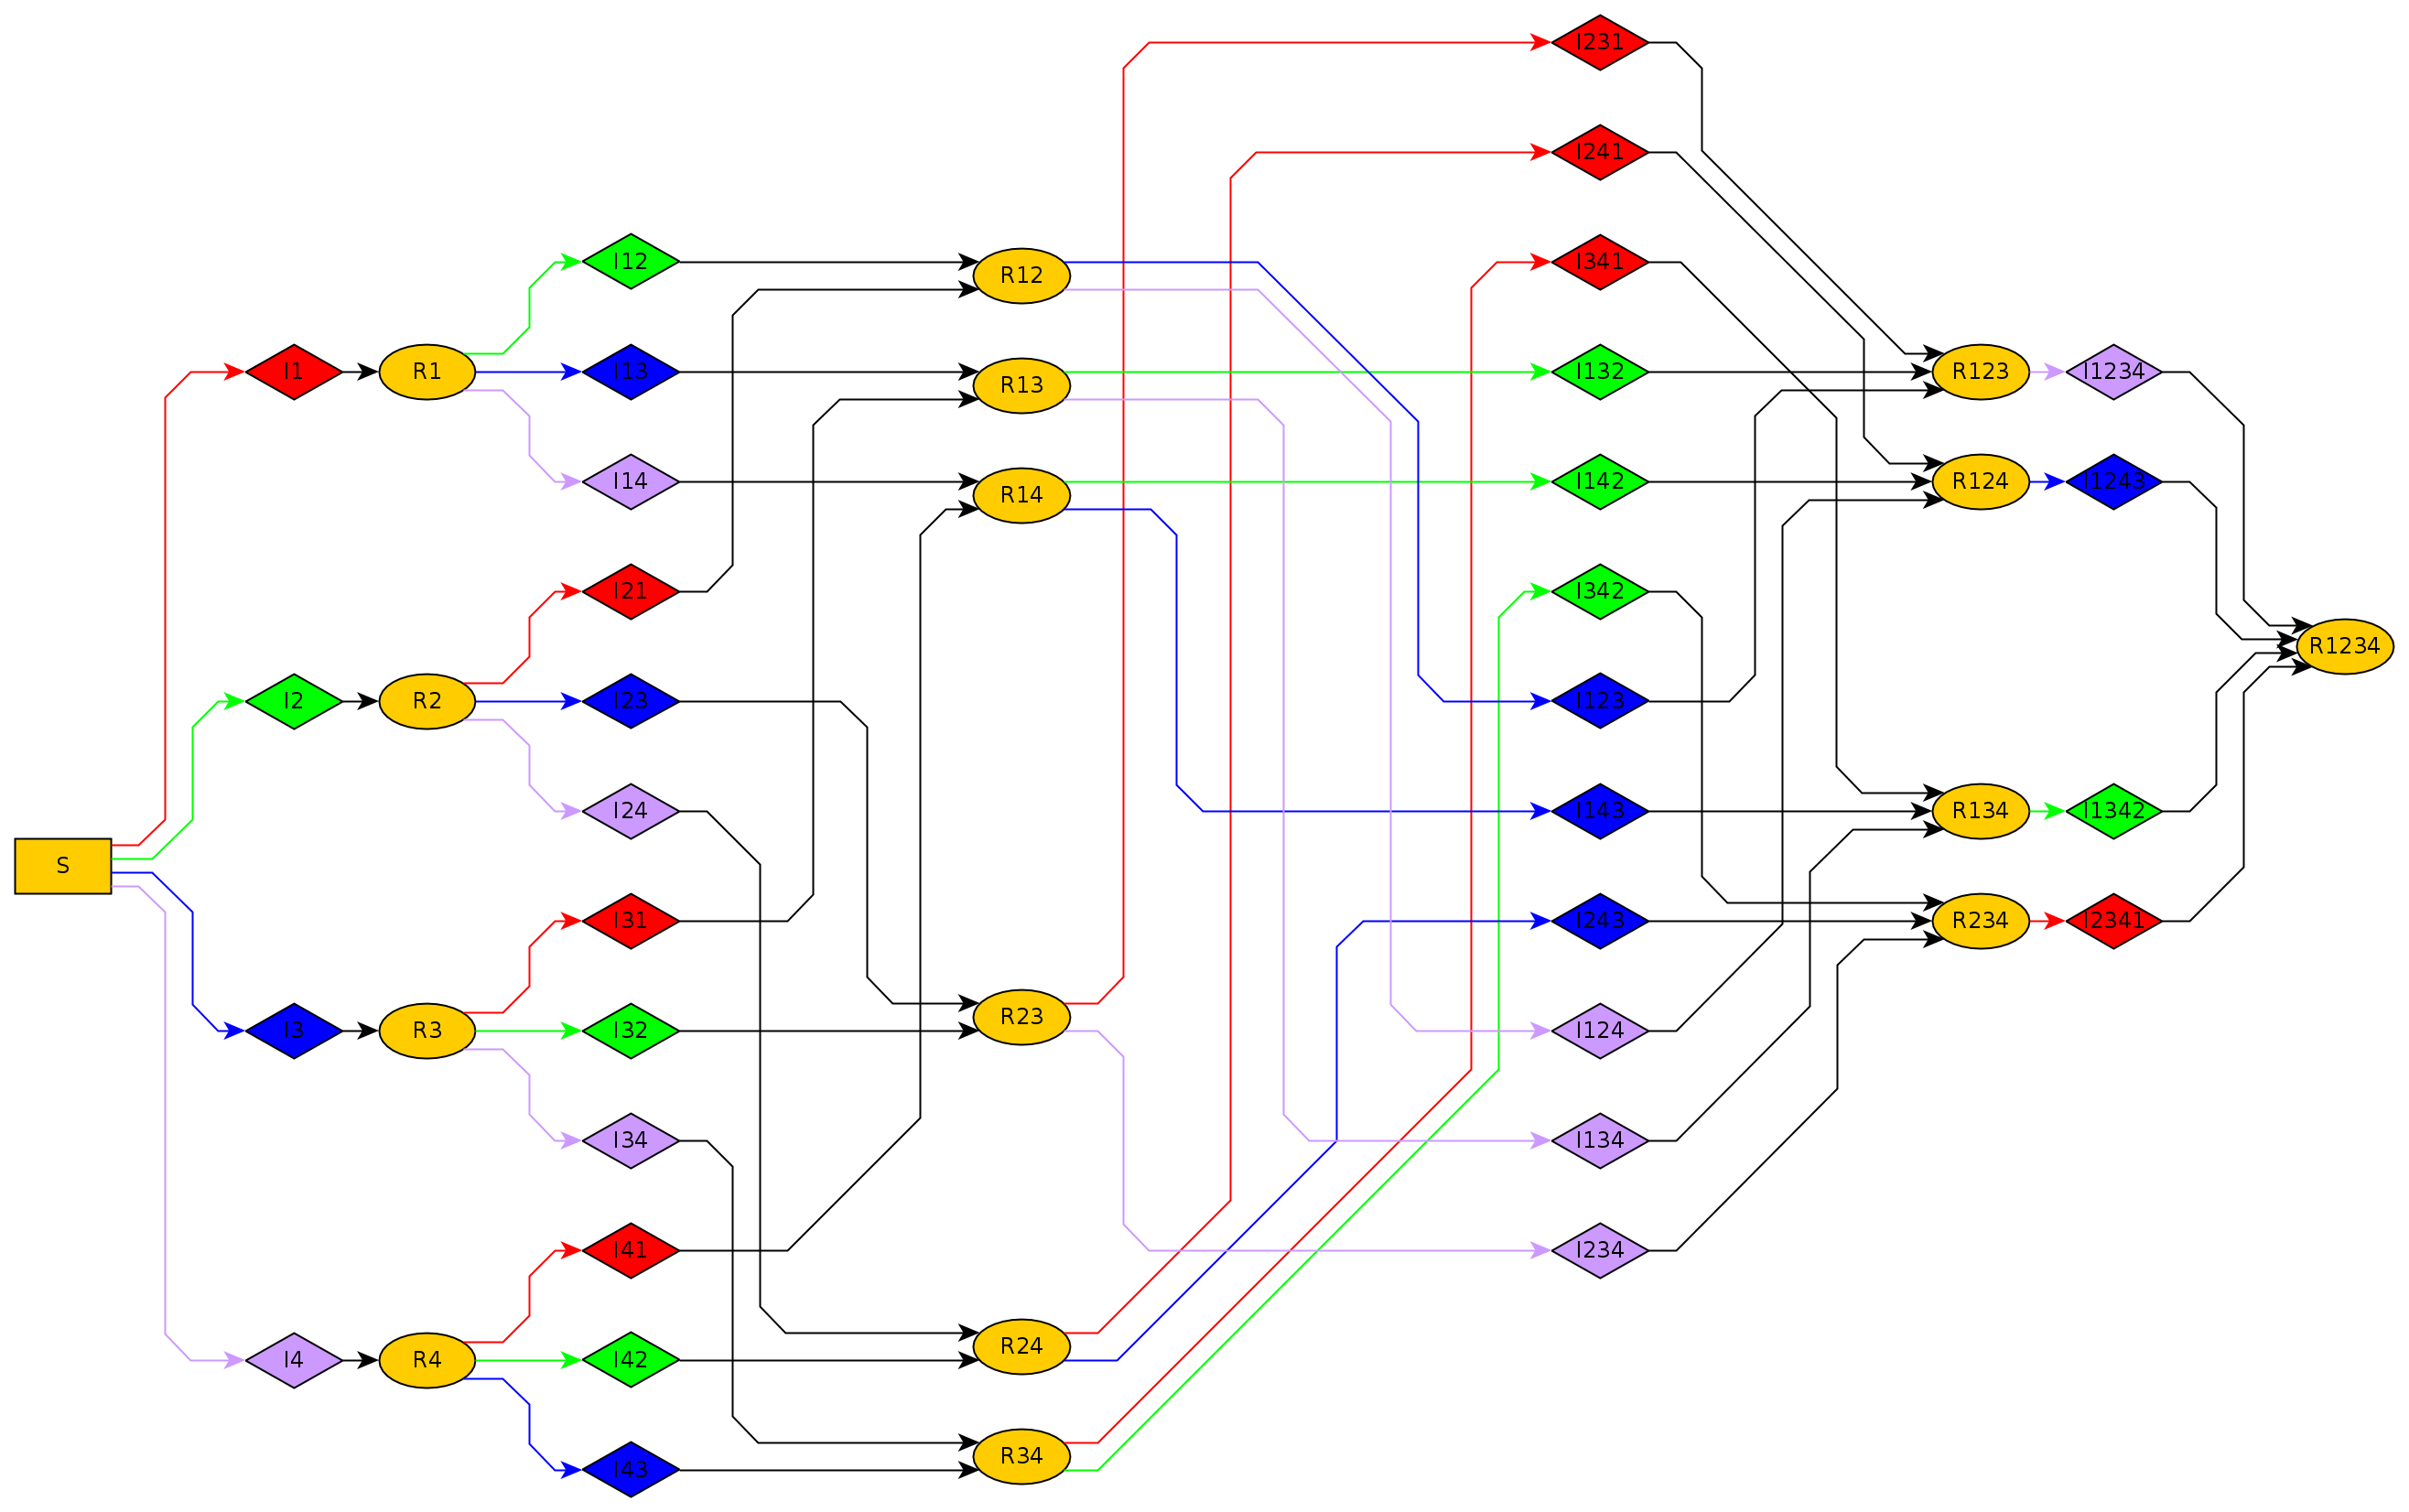
\includegraphics[width=16cm]{Dengue4.png}

 \caption{Block diagram detailing the stochastic model. Infected individuals 
with different Dengue viruses are represented by different colors. Infections 
are also represented by colored arrows matching the virus type.}
 \label{fig:sde_blocks}
\end{figure}


Let $S$ be individuals susceptible to all 4 types of dengue, $I_i$ infectious 
with Dengue type $i$ and $R_i$ individuals recovered from Dengue type $i$. 
Infectious individuals already on their secondary and later Dengue infections 
are represented by multiple indices. For example, $I_{[23]1}$ is an individual 
which has had Dengues type 2 and 3 in the past -- and therefore is immune to 
them -- and is currently transmitting Dengue 1. 
The index outside the bracket 
denotes current infection. Recovered individuals indices denote their immunity, 
so for instance $R_{123}$ is an individual which is immune to Dengue types 1, 2 
and 3, but not to 4. Let $I_{*i} = \sum I_{[\ldots]i}$ with $[\ldots]$ 
representing exposure history of the infected individual which can vary from 0 
to 3 in length. 
All individuals are born to the $S$ state and birth and death 
rates are equal.

The possible state-transitions and their  propensities are listed in table 
\ref{tab:trans}.
\begin{table}
\caption{
\bf{State-transitions and propensities: $P(\Delta X(t)|X(t))$}. The 
transitions are summarized below. Fully expanded, the system contemplates 64 
possible state transitions, as can be verified in figure \ref{fig:sde_blocks}. 
}
\label{tab:trans}
\begin{center}
\begin{tabular}[c]{l|l|l|l}
\hline
Transition & Propensity & State Change & Description\\
\hline
$S \rightarrow I_i$ & $\beta S I_{*i}$ & $\Delta S(t)=-1,\, \Delta I_i(t) = 1$ 
& Primary infection \\
$I_i \rightarrow R_i$ & $\sigma I_i$ & $\Delta I_i(t)=-1,\, \Delta R_i(t) = 1$ 
& Primary recovery\\
$R_i \rightarrow I_{[i]j}$ & $\beta \delta R_i I_{*j}$ & $\Delta R_i(t)=-1,\, 
\Delta I_{[i]j}(t) = 1$ & Secondary infection\\
$I_{[i]j} \rightarrow R_{ij}$ & $\sigma I_{[i]j}$ &$\Delta I_{[i]j}(t)=-1,\, 
\Delta R_{ij}(t) = 1$& Secondary recovery\\
$R_{ij} \rightarrow I_{[ij]k}$ & $\beta \delta R_{ij} I_{*k}$ &$\Delta 
R_{ij}(t)=-1,\, \Delta I_{[ij]k}(t) = 1$& Tertiary infection\\
$I_{[ij]k} \rightarrow R_{ijk}$ & $\sigma I_{[ij]k}$ &$\Delta 
I_{[ij]k}(t)=-1,\, \Delta R_{ijk}(t) = 1$& Tertiary recovery\\
$R_{ijk} \rightarrow I_{[ijk]l}$ & $\beta \delta R_{ijk} I_{*l}$ &$\Delta 
R_{ijk}(t)=-1,\, \Delta I_{[ijk]l}(t) = 1$& Quaternary infection\\
$I_{[ijk]l} \rightarrow R_{ijkl}$ & $\sigma I_{[ijk]l}$ & $\Delta 
I_{[ijk]l}(t)=-1,\, \Delta R_{ijkl}(t) = 1$ & Quaternary recovery\\
$\rightarrow S$ & $\mu N$ & $\Delta S = 1$ & Birth\\
$All \rightarrow$ & $\mu N$ &$\Delta All = -1$& Death\\
\hline
\end{tabular}
\end{center}

\end{table}

The model is implemented as a continuous time Markov jump process. Let
$$\overrightarrow{X}(t) = [S(t), I_1(t), I_2(t), \ldots, R_{1234}(t)]$$ 
be the 
state of the system at the time $t$. 
The system is written as a forward Kolmogorov differential equation, which in 
matrix form looks like
\begin{equation}
\frac{dP_X(t)}{dt} = Q P_X(t) 
\end{equation}

Where $P_X(t)$ is  the matrix of transition probabilities (given in table 
\ref{tab:trans}) and Q is the generator matrix, whose non-zero values are also 
given in table \ref{tab:trans} (in the state change column). The full formula 
and matrices are ommited due to their large sizes.



\bibliography{lm1}
\end{document}
